\documentclass{article}
\usepackage[inline-math]{chs-physics-report}
\usepackage{float}
\usepackage{pgfplots}
\usepackage{pgfplotstable}
\usepackage{booktabs}

\pgfplotsset{compat=1.18}

\title{2.1: Friction Lab}
\name{Gavin Chen}
\ww{Cole TerBush and Daniel Aronov}

\begin{document}
\maketitle

\section{Free Body Diagrams}
\subsection{Section 1}
\begin{center}
    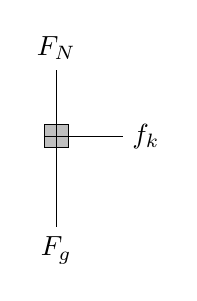
\begin{tikzpicture}[m/.style={rectangle,draw=black,fill=lightgray,minimum size=0.3cm,thin}]
        \node[m] (m) {};
        {[force,->]
        \draw (m.south) -- ++(0,-1) node[below] {$F_g$};
        \draw (m.south) -- ++(0,1) node[above] {$F_N$};
        \draw (m.west) -- ++(1,0) node[right] {$f_k$};
        }
    \end{tikzpicture}
\end{center}

\subsection{Section 2}
\begin{center}
    \begin{tikzpicture}[m/.style={rectangle,draw=black,fill=lightgray,minimum size=0.3cm,thin}]
        \node[m] (m) {};
        {[force,->]
        \draw (m.south) -- ++(0,-1) node[below] {$F_g$};
        \draw (m.south) -- ++(0,1) node[above] {$F_N$};
        \draw (m.west) -- ++(-2,0) node[left] {$f_s$};
        \draw (m.west) -- ++(2,0) node[right] {$F_{app}$};
        }
    \end{tikzpicture}
\end{center}

\subsection{Section 3}
\begin{center}
    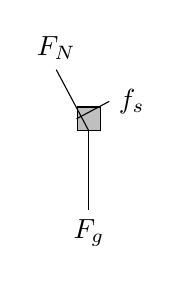
\begin{tikzpicture}[m/.style={rectangle,draw=black,fill=lightgray,minimum size=0.3cm,thin}]
        \node[m] (m) {};
        {[force,->]
        \draw (m.south) -- ++(0,-1) node[below] {$F_g$};

        \begin{scope}[rotate=28]
            \draw (m.south) -- ++(0,{cos(28)}) node[above] {$F_N$};
            \draw (m.west) -- ++({sin(28)},0) node[right] {$f_s$};

        \end{scope}
        }
    \end{tikzpicture}
\end{center}
\section{Data}
\subsection{Section 1}
\begin{center}
    \pgfplotstabletypeset[col sep=comma, /pgf/number format/fixed, fixed zerofill, precision=2, every head row/.style={
                before row={
                        \toprule
                    },
                after row={
                        \bottomrule
                    },
            },
        every last row/.style={
                after row=\bottomrule
            }]{Section 1.csv}
\end{center}

\subsection{Section 2}
\begin{center}
    \pgfplotstabletypeset[col sep=comma, /pgf/number format/fixed, fixed zerofill, precision=3, every head row/.style={
                before row={
                        \toprule
                    },
                after row={
                        \bottomrule
                    },
            },
        every last row/.style={
                after row=\bottomrule
            }]{Section 2.csv}
\end{center}

\subsection{Section 3}
\begin{center}
    \pgfplotstabletypeset[col sep=comma, /pgf/number format/fixed, fixed zerofill, precision=3, every head row/.style={
                before row={
                        \toprule
                    },
                after row={
                        \bottomrule
                    },
            },
        every last row/.style={
                after row=\bottomrule
            }]{Section 3.csv}
\end{center}
\section{$\mu$ Values}
\section{Improvements}
\end{document}